% !TEX root = ../thesis-example.tex
%
\chapter{Evaluation}
\label{sec:eval}



\begin{table}[htb]
\centering
\begin{tabular}{l|l|l}
Tagger (Trainingskorpus) & Performance(eigen) & Performance(test)  \\
\cline{1-3}
NLP4J(WSJ)  & 97.64\% & 94,86\%	\\
LingPipe(GENIA) & 96.9\% & 77,26\%	\\
FastTag(-) & - & 30,72\%          
\end{tabular}
\vspace{3mm}
\caption{Liste der Implementierten Tagger. }
\label{sec:eval:list}
\end{table}

In diesem Kapitel wird ein Test mit einem fremden Goldstandard an den implementierten Taggern ausgeführt. In Tab. \ref{sec:eval:list} sind die Per-Tag-Accuracies der Tagger aufgeführt. Performance(eigen) ist die Per-Tag-Accuracy laut eigenen Angaben (Quellen in den weiterführenden Abschnitten), Performance(test) die Per-Tag-Accuracy in diesem Test. Es ist hierbei jedoch unbedingt anzumerken, dass in diesem Test \textit{keine} Vergleiche zwischen den Taggern gezogen werden können. Hierzu müssten alle Tagger, bei denen dies möglich ist, auf den Korpus trainiert werden, um den \textit{Bias} der Tagger anzugleichen und die Ergebnisse für diesen speziellen Korpus dadurch vergleichbar zu machen.

Allerdings kann man aus einem Vergleich der eigenen Angaben mit den Testergebnissen sehen, wie stark die Performance-Änderung ist, wenn man dem Tagger einen fremden Korpus zuführt. Da auch die Trainingskorpora der Tagger sich unterscheiden, kann allerdings auch diese Änderung nicht als Vergleich zwischen den Taggern genutzt werden.

Die folgenden Abschnitte diskutieren die Auswahl eines passenden Korpus und die Performance (\textit{Scores}) der Tagger auf diesem.

\section{Goldstandard-Korpus und Aufbau des Tests}
\label{sec:eval:corpus}

Ein annotierter Korpus muss natürlich dem Tagset der einzelnen zu testenden Tagger entsprechen. Zudem sollte aus dem Goldstandard direkt die Sequenzierung auslesbar sein, da sonst Tokenization stattfinden müsste und Sequenzierungsunterschiede die Ergebnisqualität der Tagger trüben könnten.

Ein Korpus, der beiden Kriterien entspricht, ist die \textit{NAIST/NTT TED Treebank} \cite{tedbank}. Alle Inhalte sind sowohl als \textit{Tokenized} (Token getrennt durch Leerzeichen und Zeilenumbrüche) als auch annotiert nach derselben Sequenzierung verfügbar. Die zur POS-Tag-Evaluation überflüssigen Syntaxbaum-Tags können einfach ignoriert werden. Die Notation des Annotierten Textes entspricht der Klammer-Notation  aus Abschnitt \ref{sec:impl:eval:parsing} und kann somit vom Parser des Evaluationsoperators erkannt werden.

Im Rahmen des Tests wird diese Treebank verwendet. Der RapidMiner-Prozess zum Testen ist in Abb. \ref{fig:eval:corpus:process} dargestellt. Für die nachfolgenden Tests wurden sämtliche Teilstücke des Testkorpus eingelesen und zu einem Dokument aneinandergereiht. Zur Übersichtlichkeit wurde in der Abbildung allerdings nur einfaches Einlesen von einem Teilstück modelliert. 

\begin{figure}[htb]
	\centering
	\captionsetup{justification=centering,margin=2cm}
	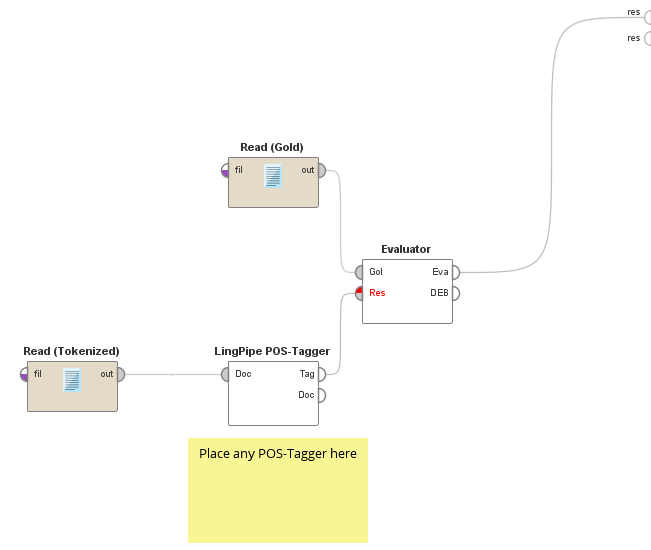
\includegraphics[width=0.7\textwidth]{gfx/process.png}
	
	\caption{Aufbau des Test-Evaluationsprozesses} 
	\label{fig:eval:corpus:process}
\end{figure}

Der LingPipe-Tagger im Prozess hat identische Inputs und Outputs zu den anderen Taggern, und kann hier einfach ersetzt werden. Die Einlese-Operatoren lesen für den Tagger die sequenzierten Texte mit der Dateiendung \textsc{.tok} und als Goldstandard die annotierten Texte in Klammer-Format mit Endung \textsc{.mrg}. Der Evaluationsoperator \textit{Evaluator} wird auf diese Formatierung konfiguriert.

\section{Evaluation der einzelnen Tagger}
\label{sec:eval:detail}

\subsection{NLP4J (WSJ)}
\label{sec:eval:detail:nlp4j}

\begin{table}[htb]
\centering
\captionsetup{justification=centering,margin=2cm}
\begin{tabular}{l|l}
Metrik & Performance \\
\cline{1-2}
Per-Tag-Accuracy & 94,86\%\\
Per-Sentence-Accuracy & 49,19\%\\
\cline{1-2}
Precision(NN) & 96,11\%\\
Recall(NN) & 96,85\%\\
F-Score(NN) & 96,48\%\\
\cline{1-2}
Precision(VBD) & 95,11\%\\
Recall(VBD) & 95,7\%\\
F-Score(VBD) & 95,4\%
\end{tabular}
\vspace{3mm}
\caption{Scores des NLP4J-Taggers (Training: WSJ-Korpus)}
\label{tab:eval:detail:nlp4j}
\end{table}

Der NLP4J-Tagger erreicht gemäß der Werte in Tab. \ref{tab:eval:detail:nlp4j} beinahe seine maximale Leistungsfähigkeit(97.64\% \cite{choi}). Daraus lässt sich schließen, dass der \textit{Bias} in Richtung des WSJ-Korpus, auf dem trainiert wurde, zu keinen sehr hohen Performanceverlusten beim Testkorpus führt, also eine hohe Ähnlichkeit zwischen den Korpora herrscht. Alternativ könnte der NLP4J-Tagger auch hochgradig unanfällig gegen Bias sein, allerdings müssten für solch eine Aussage mehr Tests stattfinden. 

Auffällig ist die Per-Sentence-Accuracy von knapp 50\%, jedoch klärt eine kurze Rechnung das schnell auf: Bei einer Wahrscheinlichkeit von 94,86\% und einer (angenommenen) durchschnittlichen Satzlänge von 13 Wörtern beträgt die Wahrscheinlichkeit, dass der Satz vollständig korrekt ist (also dass 13 Wörter in Folge korrekt sind) $0,9486^{13}\approx 50,36\% $. Bei den eingelesenen 23.158 Wörtern und 1.486 daraus gelesenen Sätzen beträgt die tatsächlich durchschnittliche Satzlänge $\frac{23.158}{1.486}\approx 15.58 $. Die kleine Diskrepanz von 2,58 Worten zwischen Annahme und Ergebnis lässt sich mit der ungleichen Verteilung der Satzlängen im Korpus erklären. Dies wird hier nicht weiter überprüft, aber da der Korpus aus Untertiteln von \textit{TED Talks}, also Reden entnommen ist, erscheint das plausibel.


\subsection{LingPipe (GENIA)}
\label{sec:eval:detail:lingpipe}

\begin{table}[htb]
\centering
\captionsetup{justification=centering,margin=2cm}
\begin{tabular}{l|l}
Metrik & Performance \\
\cline{1-2}
Per-Tag-Accuracy & 77,26\%\\
Per-Sentence-Accuracy & 10,96\%\\
\cline{1-2}
N-Accuracy(n=5) & 77,32\%\\
N-Distanz(n=5) & 2,134\\
\cline{1-2}
Precision(NN) & 62,65\%\\
Recall(NN) & 77,42\%\\
F-Score(NN) & 69,25\%\\
\cline{1-2}
Precision(VBD) & 81\%\\
Recall(VBD) & 73,36\%\\
F-Score(VBD) & 76,99\%
\end{tabular}
\vspace{3mm}
\caption{Scores des LingPipe-Taggers (Training: GENIA Korpus)}
\label{tab:eval:detail:lingpipe}
\end{table}

In Tab. \ref{tab:eval:detail:lingpipe} finden sich die Scoring-Ergebnisse des Ling-Pipe Taggers, konfiguriert mit den Trainingsergebnissen auf Basis des GENIA Korpus. Laut Tests in \cite{Lingpipeeval} erreicht LingPipe eine Per-Tag-Accuracy von bis zu 96.9\%. Diese wurde hier bei weitem nicht erreicht. Allerdings ist der GENIA Korpus, auf dem trainiert wurde, eine Sammlung an biomedizinischem Fachwissen, daher ist die Leistungsminderung verständlich. 

Besonders an diesem Tagger ist, dass er potenziell n beste Tags pro Token ausgibt, daher wurde hier eine N-Accuracy und N-Distanz für n = 5 berechnet. Allerdings fällt bei Inspektion des TagStrings auf, dass die 5 Tags pro Token in diesem Fall fast immer identisch waren (es liegt die Vermutung nahe, dass das zugrundeliegende Modell nicht zu mehr Differentiation in der Lage war). Daher ist die N-Accuracy nur marginal höher und die N-Distanz ist nahe dem Minimum von $(n+1)-Accuracy*n\approx 6-0,7726*6=2,13$.

\subsection{FastTag}
\label{sec:eval:detail:fasttag}

\begin{table}[htb]
\centering
\captionsetup{justification=centering,margin=2cm}
\begin{tabular}{l|l}
Metrik & Performance \\
\cline{1-2}
Per-Tag-Accuracy & 30,72\% \\
Per-Sentence-Accuracy & 0,87\%\\
\cline{1-2}
Precision(NN) & 15,92\%\\
Recall(NN) & 89,39\%\\
F-Score(NN) & 27,02\%\\


\end{tabular}
\vspace{3mm}
\caption{Scores des FastTag-Taggers}
\label{tab:eval:detail:fasttag}
\end{table}

FastTag erreicht nur eine extrem niedrige Accuracy. Um diese zu erklären, können wir einen Blick auf die Confusion-Matrix-Metriken für das Tag NN werfen: Es fällt sofort auf, dass der Recall-Wert ungewöhnlich hoch ist. Der Tagger rät bei Wörtern, die nicht im Lexikon vertreten sind, immer das Tag \textsc{NN}. Ein hoher Recall bedeutet, dass viele der NN-Tags im Goldstandard erkannt wurden. Auf der anderen Seite sagt die niedrige Precision jedoch aus, dass viele der geratenen NN falsch waren. Es wird also erkennbar, dass dieser Taggingprozess durch viele Rateversuche gekennzeichnet war und vor allem an einem zu kleinen Lexikon gescheitert ist. Zusätzlich verwendet FastTag auch keinerlei Worttransformationsmethoden, die dieses Problem verhindern könnten.

Die Metriken für das Tag \textsc{VBD} wurden ausgelassen, da der Tagger dieses Tag nicht verwendet.

\section{Zusammenfassung}
\label{sec:eval:conclusion}

Bereits die Testergebnisse aus dieser überschaubaren Untersuchung liefern einen hohen Informationsgehalt. Es lässt sich beobachten, wie extrem sich der Bias der beiden trainierten POS-Tagger auf deren Scores auswirkt.

